\chapter{Chapter Two}
\section{Methodology}
\subsection{Comparison of Radar Systems}
Comparing two radar datasets is fraught with challenges; solutions to meet this challenge are presented herein. Even though the radar system characteristics are not identical, the measurements are comparable due to the design of the weather radar equation, which accounts for the sensitivity of the radar system itself \citep{Rogers1989}. The area of study was chosen to ensure that the coinciding radar scans had similiar resolution samples and beam heights. 
\begin{figure}[h]
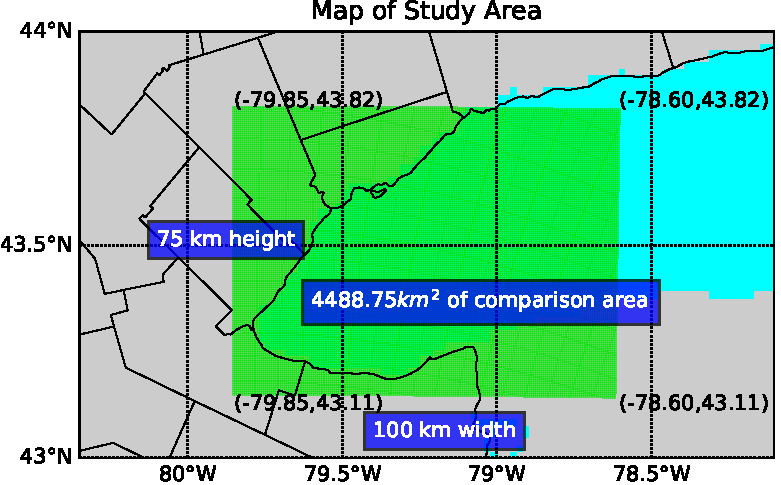
\includegraphics[]{study_area}\centering
\caption{Bounding box of the study area, denoted by the green shading. (latitude, longitude) given for each corners.} 
\label{fig:study_area}
\end{figure}
Lake Ontario happens to be the perfect area to bound between the radars, therefore only data from areas over water inside the bounding box depicted in Figure \ref{fig:study_area} are used. This also ensures that no ground clutter is incorporated into the analyses.
\subsubsection{Comparing Radar Characteristics}

As presented in Equation \ref{eq:weather_eq}, the weather radar equation is defined by constant parameters dependent on the radar system characteristics, and varying properties related to the target. 
\begin{equation}\label{eq:weather_eq}
\bar{P_r} = \frac{\pi^3c}{1024 \ln(2)} \Bigg[\frac{P_t \tau G^2 \theta^2}{\lambda^2}\Bigg]_{dBZ_0} \Bigg[|K^2|\frac{Z_{eH}}{r^2}\Bigg]_{TARGET}
\end{equation}
The target properties are dielectric constant (K), range (r) and equivalent reflectivity factor $Z_{eH}$. Conversely, the radar parameters ideally remain unchanged from their values upon installation of the radar system. These parameters form the radar constant, symbolically expressed as $dBZ_0$. The parameters that define this constant include the power transmitted ($P_t$), the pulse length ($\tau$), the antenna gain (G), the angular beamwidth ($\theta$), and the wavelength ($\lambda$).
\begin{equation}\label{eq:radpow}
10 \log Z = 10 \log{\bar{P_r}} + 20 \log r - dBZ_0
\end{equation}

Equation \ref{eq:radpow} shows how $dBZ_0$ is subtracted out from the full calculation of $Z$. Table \ref{radarspecs} compares these parameters for both radar systems. The biggest difference between the two is the wavelength, with CWKR operating in the C frequency band and KBUF operating in the S frequency band. It should be noted that although KBUF has a larger physical beamwidth than CWKR, it achieves an effective azimuthal resolution of $0.5^{\circ}$ through an over-sampled data windowing technique \citep{Torres2007}. Therefore, the two radars are matched in azimuthal resolution, while CWKR has twice the range resolution of KBUF. Also, it should be stated that the signal processors used in both radar systems are in the Vaisala SIGMET series, therefore they measure $Z_{eH}$ and $Z_{DR}$ using 8 bit resolution. With data intervals of -31.5 dBZ to +95.5 dBZ and -7.94 dB to +7.94 dB, This equates to a data resolution of 0.5 dBZ and 0.0625 dB, respectively.

\begin{table}[h]
    \caption{Specifications of each radars system, with symbols as used in Eq. \ref{eq:radpow}}\label{radarspecs}
    \begin{center}
    \begin{tabular}{|l|c|c|}
    \hline
     field [symbol](unit) & King City (CWKR) & Buffalo (KBUF) \\
    \hline\hline
    Wavelength [$\lambda$](cm) & 5 (C-Band) & 10 (S-Band) \\
    \hline
    Beamwidth [$\theta$] ($^\circ$)  & 0.62  & 0.92 \\
    \hline
     Antenna Gain [G] (dB) & 45.5 & 49.2 \\
    \hline
     Transmitter Peak Power (kW) & 250 & 1000 \\
    \hline
     Pulse Length [$\tau$] ($\mu s$) &  0.8/2.0 & 1.5/4.5 \\
    \hline
     Matched Elevation Angle ($^\circ$) & 0.2 & 0.5 \\
    \hline
     Range Resolution [$r$] (m)& 125 & 250 \\
    \hline
    \end{tabular}
    \end{center}
\end{table}


\subsection{Distance-Weighting Scheme}
The biggest challenge when comparing radar resolution volumes measured by radars that are not co-located is resolving the differences in coordinate system. A resolution volume is defined as volume irradiated by the idealized Gaussian beam pattern for each range gate, otherwise known as a bin. Resolution volumes are sampled natively in the spherical coordinate system; although there may be some overlap, the shape of the bins will vary drastically. Differences between KBUF and CWKR bin geometry can be ascertained from Figure \ref{fig:compare_bins}. 
\begin{figure}[H]
\centering
   \begin{subfigure}{1.0\textwidth} \centering
     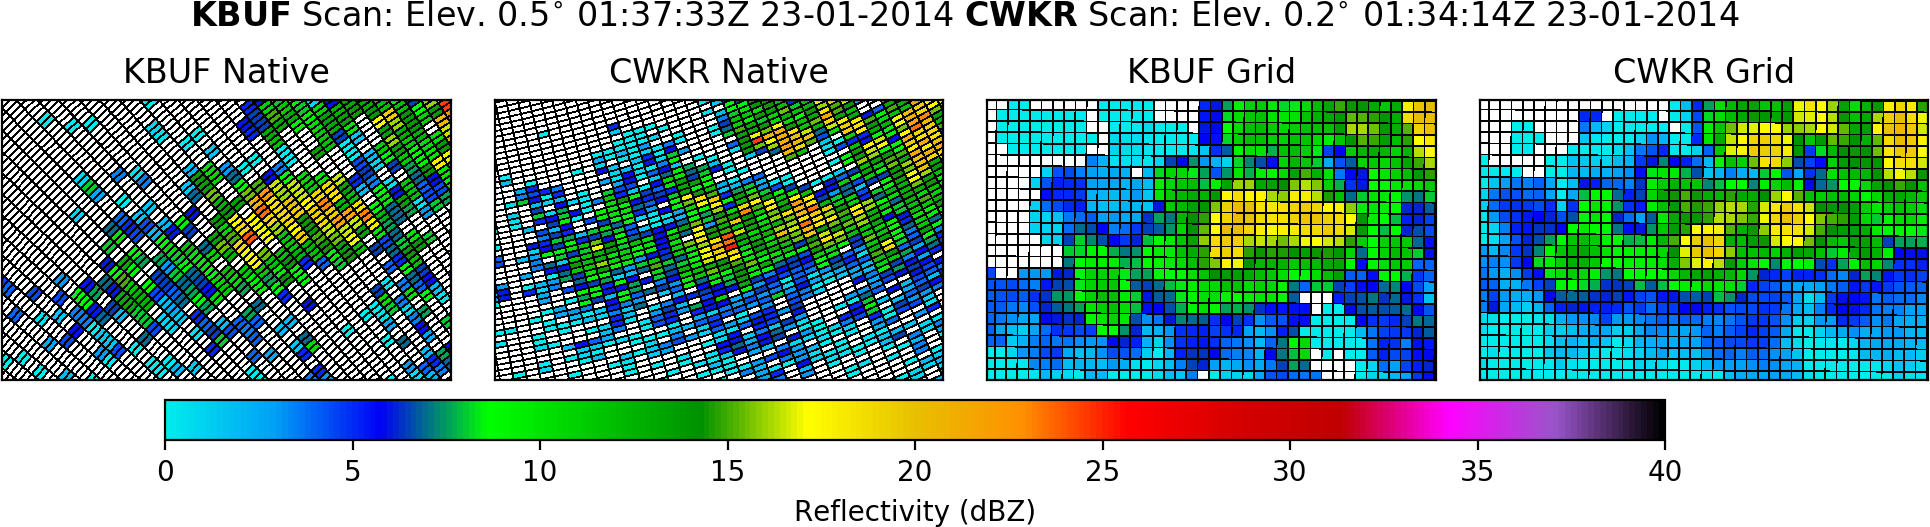
\includegraphics[width=1\linewidth]{compare_bins_ref}
     \caption{$Z_H$ comparison, shows the smooth transformation from an isotropic input to an isotropic gridded output.}\label{fig:compare_ref}
   \end{subfigure}
   \begin{subfigure}{1.0\textwidth} \centering
     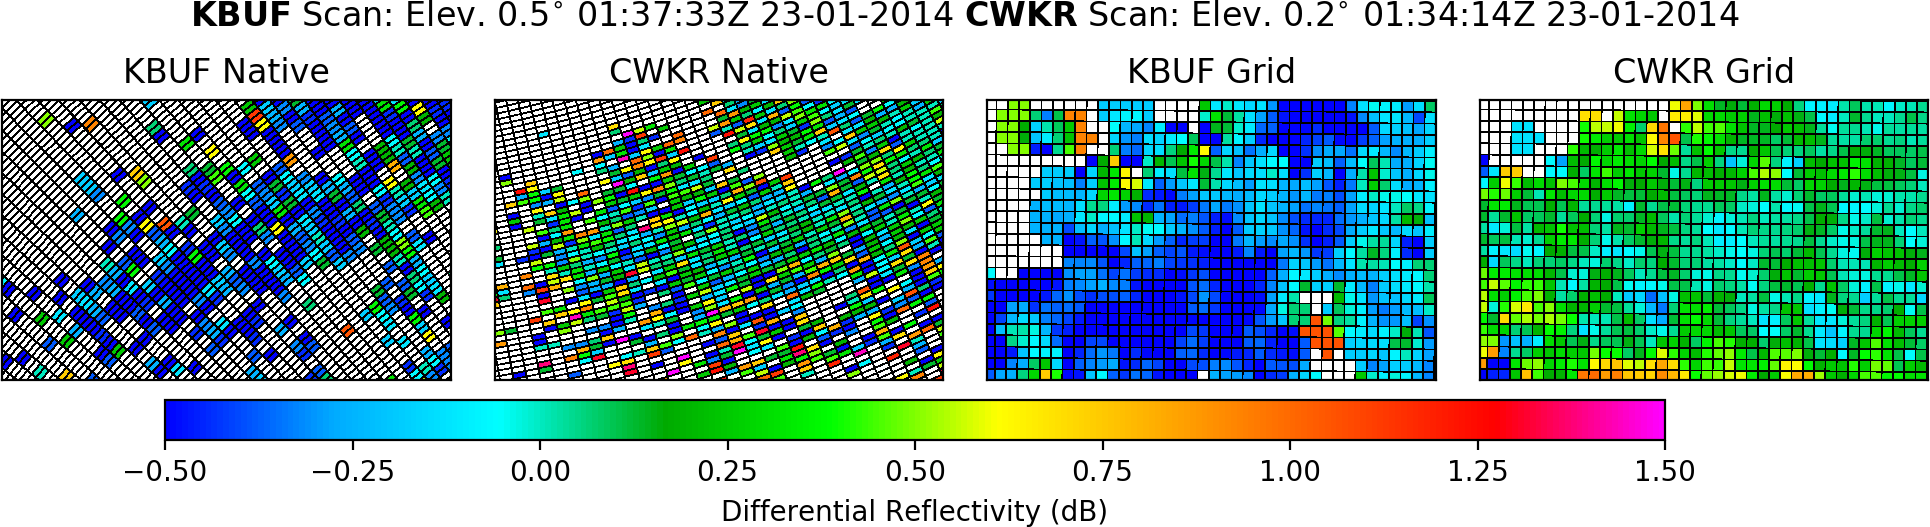
\includegraphics[width=1\linewidth]{compare_bins_zdr}
     \caption{$Z_{DR}$ comparison, in contrast with (a), shows the limitations of representing an anisotropic field with an isotropic distance-weighting function. }\label{fig:compare_zdr}
   \end{subfigure}
\caption{Base moment comparisons between radars over Lake Ontario, with dimensions of 20x12.5 km. Left panels are in native radars coordinates, with gates outlined in black. Right panels are transformed to a common Cartesian grid, with grid cells outlined in black.} \label{fig:compare_bins}
\end{figure}
These differences require the radar data to be objectively analyzed onto a common coordinate system, which can be achieved through a distance-weighting scheme. This method was adopted in the open source software module called the Python ARM Radar Toolkit (Py-ART) \citep{Py-ART}, which is used here. In accordance with the recommendations of \cite{Pauly1990}, a grid resolution ($\Delta x$, $\Delta y$) of 500 meters is chosen. A Barnes distance-weighting scheme is used for this analysis. 
\begin{equation}\label{eq:barnesdws}
f^{'}_{p} = \sum_{b=1}^n  e^{-(d_b/\kappa)^{2}} f_q  \bigg/ \sum_{b=1}^n e^{-(d_b/\kappa)^{2}}
\end{equation}
The Gaussian weighting function used in said scheme is given in Equation \ref{eq:barnesdws}. It shows that the value of the analysis at some point $p$ is equal to sum of weights convolved with the actual values at bin $b$ in radar space, divided by the sum of the weights. The summation is performed over $n$ number of bins that are within the radius of influence ($\kappa$) of the center point of the grid cell, and d is is the horizontal distance from the native bin to the center point of the cell. Vertical distance is neglected, as only the lowest elevation angle from the radars are included for comparison.
\begin{equation}\label{eq:roi}
\kappa = D * \tan{\theta}
\end{equation}
The definition of $\kappa$ is found in Equation \ref{eq:roi}, where D is the horizontal distance from the grid cell to the radar and $\theta$ is the angular beamwidth. This completes the framework for comparing the radar datasets in this study.
\section{Selection of Cases}
\begin{table}[h]
    \caption{Critical level temperatures from radiosonde launched closest in time to the selected lake-effect snow events.}\label{eventslake}
    \begin{center}
    \begin{tabular}{|l|c|c|c|}
    \hline
     KBUF - Radiosonde & Radar Times & 850mb T ($^{\circ}C$) & Lowest-Level T ($^{\circ}C$)\\
    \hline\hline
    2014-01-23 00Z & 0100-1000Z & -22.5 & -14.9 \\
    \hline
    2015-01-06 12Z & 1200-1700Z & -20.1 & -11.7 \\
    \hline
    2015-02-14 12Z & 1000-1400Z & -14.9 & -6.9 \\
    \hline
    2015-02-18 12Z & 2100-2359Z & -17.3 & -10.1 \\
    \hline
    2016-02-10 12Z & 1300-2359Z & -10.5 & -2.7 \\
    \hline
    \end{tabular}
    \end{center}
\end{table}
\begin{table}[h]
    \caption{Critical level temperatures from radiosonde launched closest in time to the selected synoptic snow events.}\label{synopticevents}
    \begin{center}
    \begin{tabular}{|l|c|c|c|}
    \hline
     KBUF - Radiosonde & Radar Times & 850mb T ($^{\circ}C$) & Lowest-Level T ($^{\circ}C$)\\
    \hline\hline
    2014-01-18 12Z & 0600-0800Z & -11.3 & -6.5 \\
    \hline
    2015-01-07 12Z & 0900-1100Z & -20.1 & -11.7 \\
    \hline
    2015-02-06 12Z & 0900-1030Z & -16.3 & -10.7 \\
    \hline
    2016-01-06 12Z & 0700-0900Z & -7.5 & -0.7 \\
    \hline
    2016-12-15 12Z & 0920-1020Z & -20.3 & -12.3 \\
    \hline
    \end{tabular}
    \end{center}
\end{table}
Cases selected for this study were chosen entirely based on the pattern of motion and banding of the radar echoes. Radar mosaics for the study area were manually examined, beginning in 2014. When time intervals with echoes in the study area were observed, it was noted whether they trained over the same area, or were progressive. The former are classified as lake-effect driven events, while the latter are synoptically driven events. Also, a tabulation of critical level temperatures for the five lake-effect snow events selected is shown in Table \ref{eventslake}, while the synoptic events are shown in Table \ref{synopticevents}. This shows ensures that all events were sufficiently below freezing, and dry snow was the predominant hydrometeor type.
\section{Filtering Conditions}
Several conditions were used to narrow down the selected sets to the best suited scans and individual gates for admission into the distance-weighting scheme.
\subsection{Time Filter}
Scan start times are compared between the radars, and if they are within four minutes of each other, the pair is admitted. For CWKR, there is a regular volume update frequency of ten minutes, while KBUF is variable based on the Volume Coverage Pattern (VCP) selected by the operator. The update frequency could be as short as every two minutes if the operator has activated Supplemental Adapative Intra-Volume Low-Level Scans (SAILS) mode.
\subsection{Gate Filters}

\section{Advanced Statistical Techniques}
Scatter plots directly comparing grid cells produced by the distance-weighting scheme are used in this study. This section discusses how advanced statistical techniques were leveraged to derive the most information from these plots.
\subsection{Kernel Density Estimation}

Large radar datasets contain an immense amount of data; this requires the distillation of data to the greatest statistical significance. Scatter-plots containing on the order of $10^5$ points become visually overwhelming. To solve this problem, a Kernel Density Estimation (KDE) technique is used. A 2-D KDE is essentially a way to estimate the joint probability density function of two random variables \citep{Silverman1986}. Figure \ref{fig:synthetic_KDE} demonstrates how this is achieved graphically, by first solving each individual kernel, then performing a summation. The units of the KDE can be thought of as a likelihood ratio. Furthermore, the units are normalized by the matrix in Equation \ref{eq:norm_kde}, where \textbf{X} represents a 2-D histogram of the matched cells, $n$ is the number of matched cells, and $R$ is the histogram bin resolution, which matches the native data resolution.
\begin{equation}\label{eq:norm_kde}
\mathbf{N}_{i,j} = n * R^{2} * \sqrt{\mathrm{Det} \vert 2\pi * \mathrm{Cov}(\mathbf{X_{i}},\mathbf{X_{j}}) * n^{-1/6} \vert}
\end{equation}
\begin{figure}
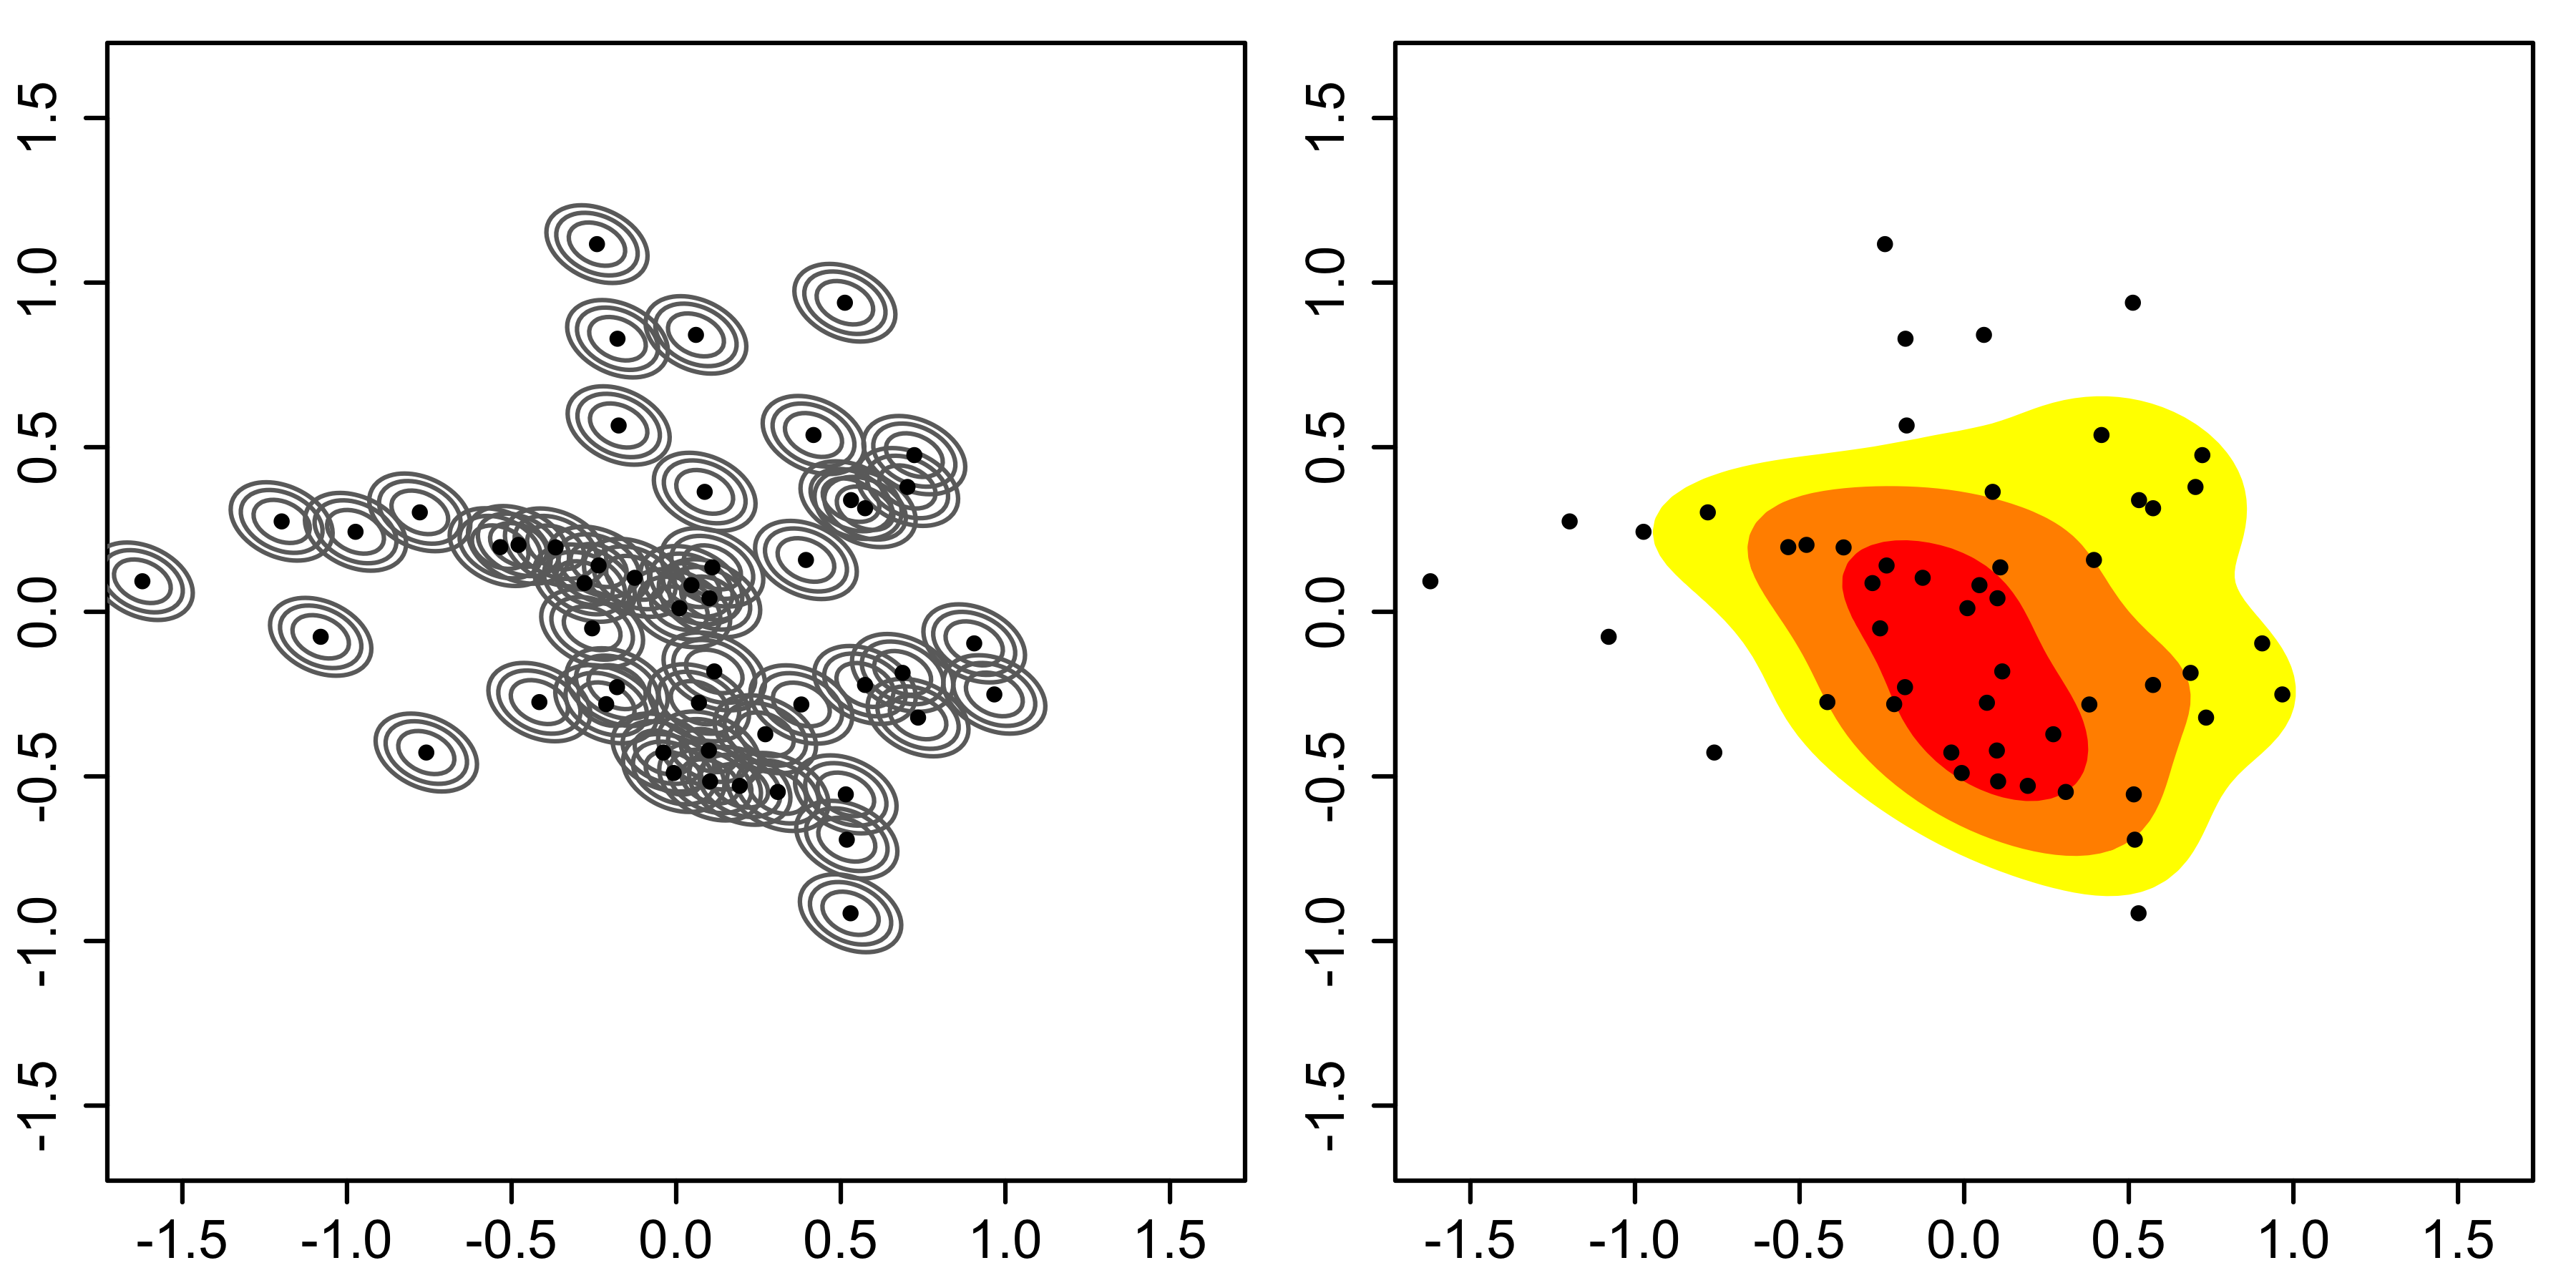
\includegraphics[scale=0.1]{Synthetic_data_2D_KDE}\centering
\caption{Illustration of the construction of 2D kernel density estimates. (Left) data points with individual kernels as grey dashed lines, (right) summed kernels = kernel density estimate.} 
\label{fig:synthetic_KDE}
\end{figure}

\subsection{Orthonormal Linear Regression}
\begin{figure}
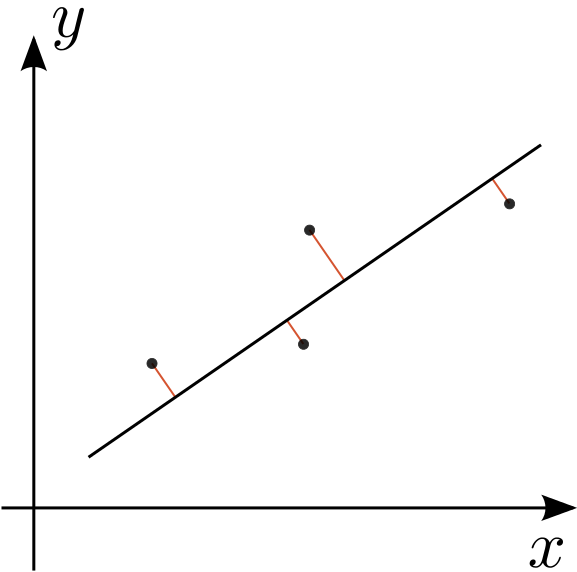
\includegraphics[scale=0.4]{total_least_square}\centering
\caption{Demonstration of an Orthonormal Linear Regression} 
\label{fig:total_least_squares}
\end{figure}
A hallmark of this study is the lack of ground truth. The sample sets compared, \textbf{K} and \textbf{C}, contain error prone, independent variables. Typically, scatter-plots compare an independent variable to a dependent variable. Instead of performing a standard linear regression between the variables, an orthonormal linear regression is used. This type of regression allows for error in both variables, by performing the least squares regression perpendicular to the initial fit instead of vertically \citep{Markovsky2007}. Figure \ref{fig:total_least_squares} demonstrates this concept.

\section{$Z_{DR}$ Bias Estimation}
Although it not possible to check absolute calibration of $Z_{eH}$ when comparing two radars, it is possible to verfiy $Z_{DR}$ calibration due to relative nature of the quantity \citep{Zrnic2006}.
While radars are regularly calibrated using internal calibration procedures, an external check is useful for monitoring the time-varying component of calibration. The typical process for calibration of $Z_{DR}$ is pointing the antenna to zenith and performing ``bird bath'' scans during light rain events \citep{Hubbert2006}. The $Z_{DR}$ in light rain is expected to be 0 dB, therefore any offset from this is considered a bias; The signal processor subtracts out this bias to achieve the final output. Due to mechanical constraints, NEXRAD radars are unable to perform this procedure, but CWKR is (citation needed). NEXRAD radars disseminate a product which contains an estimate of $Z_{DR}$ bias using the intrinsic properties of dry snow \cite{Zittel2015}. The daily published offset will be used to adjust $Z_{DR}$ values obtained from KBUF to diagnose any bias at CWKR.



